\documentclass[12pt, twoside]{article}
\usepackage{jmlda}
\usepackage{graphicx}
\newcommand{\hdir}{.}

% notations
% bold
\newcommand{\bz}{\mathbf{z}}
\newcommand{\bx}{\mathbf{x}}
\newcommand{\by}{\mathbf{y}}
\newcommand{\bw}{\mathbf{w}}
\newcommand{\bfx}{\mathbf{f}}
\newcommand{\bb}{\mathbf{b}}
\newcommand{\bu}{\mathbf{u}}
\newcommand{\bh}{\mathbf{h}}
\newcommand{\bX}{\mathbf{X}}
\newcommand{\bZ}{\mathbf{Z}}
\newcommand{\bA}{\mathbf{A}}
\newcommand{\bI}{\mathbf{I}}
\newcommand{\bJ}{\mathbf{J}}
\newcommand{\bV}{\mathbf{V}}
\newcommand{\bU}{\mathbf{U}}
\newcommand{\bG}{\mathbf{G}}
\newcommand{\btheta}{\boldsymbol{\theta}}
\newcommand{\bPsi}{\boldsymbol{\Psi}}
\newcommand{\bpsi}{\boldsymbol{\psi}}
\newcommand{\bxi}{\boldsymbol{\xi}}
\newcommand{\bchi}{\boldsymbol{\chi}}
\newcommand{\bzeta}{\boldsymbol{\zeta}}
\newcommand{\blambda}{\boldsymbol{\lambda}}
\newcommand{\beps}{\boldsymbol{\varepsilon}}
\newcommand{\bZeta}{\boldsymbol{Z}}
\newcommand{\bg}{\mathbf{g}}
\newcommand{\bff}{\mathbf{f}}
\newcommand{\bv}{\mathbf{v}}
% mathcal
\newcommand{\cX}{\mathcal{X}}
\newcommand{\cY}{\mathcal{Y}}
\newcommand{\cW}{\mathcal{W}}
\newcommand{\cL}{\mathcal{L}}
% transpose
%\newcommand{\T}{^{\mathsf{T}}}
%other
\newcommand{\fD}{\mathfrak{D}}
\newcommand{\fG}{\mathfrak{G}}
\newcommand{\fF}{\mathfrak{F}}
\newcommand{\bbR}{\mathbb{R}}
\newcommand{\bbY}{\mathbb{Y}}

\begin{document}

\title
    [Оптимизация параметров модели на основе дистилляции знаний] % краткое название; не нужно, если полное название влезает в~колонтитул
    {Регуляризация траектории оптимизации параметров модели глубокого обучения на основе дистилляции знаний}
\author
    [М.~Горпинич] % список авторов (не более трех) для колонтитула; не нужен, если основной список влезает в колонтитул
    {М.~Горпинич, О.\,Ю.~Бахтеев, В.\,В.~Стрижов} % основной список авторов, выводимый в оглавление
    [М.~Горпинич, О.\,Ю.~Бахтеев, В.\,В.~Стрижов] % список авторов, выводимый в заголовок; не нужен, если он не отличается от основного
\email
    {gorpinich4@gmail.com; bakhteev@phystech.edu;  strijov@ccas.ru}
%\thanks
%    {Работа выполнена при
%     частичной
%     финансовой поддержке РФФИ, проекты \No\ \No 00-00-00000 и 00-00-00001.}
%\organization
%    {$^1$Организация, адрес; $^2$Организация, адрес}
\abstract
    {Исследуется задача оптимизации параметров модели глубокого обучения. Предлагается обобщение методов дистилляции, заключающееся в градиентной оптимизации гиперпараметров. На первом уровне оптимизируются параметры модели, на втором --- гиперпараметры, задающие вид оптимизационной задачи. Исследуются свойства оптимизационной задачи и различные виды оператора оптимизации. Предложенное обобщение позволяет производить дистилляцию модели с лучшими эксплуатационными характеристиками и за меньшее число итераций оптимизации. Проиллюстрирована комбинация данных подходов с помощью вычислительного эксперимента на выборке CIFAR-10.
	
\bigskip
\noindent
\textbf{Ключевые слова}: \emph {machine learning; knowledge distillation; hyperparameter optimization; recurrent neural network}
}

%данные поля заполняются редакцией журнала
\doi{}
\receivedRus{}
\receivedEng{}

\maketitle
\linenumbers

\section{Введение}
В работе исследуется проблема оптимизации моделей глубоких нейросетей. Данная задача требует значительных вычислительных мощностей и является затратной по времени. В данной работе предлагается метод оптимизации, позволяющий улучшить эксплуатационные характеристики модели, а также ускорить ее сходимость к точке оптимума.

Предлагается обобщение метода оптимизации на основе дистилляции знаний. Рассматривается \textit{модель-учитель} более сложной структуры, которая была обучена на выборке. Модель более простой структуры предлагается оптимизировать путем переноса знаний модели учителя на более простую модель, называемую \textit{моделью-учеником}, при этом ее качество будет выше по сравнению с качеством, полученным после оптимизации на той же выборке. Данный подход описан в \cite{journals/corr/HintonVD15}. В \cite{conf/cvpr/PassalisTT20} предложен подход к дистилляции знаний, переносящий знания на модель с архитектурой, значительно отличающейся от архитектуры модели-учителя.

Предлагается представление задачи в виде двухуровневой оптимизации. На первом уровне оптимизируются параметры модели, на втором уровне --- ее гиперпараметры. Данный подход описан в \cite{journals/corr/LuketinaBR15, journals/anor/BakhteevS20, journals/corr/MaclaurinDA15}. В \cite{journals/corr/LuketinaBR15} рассматривается жадный градиентный метод оптимизации гиперпараметров. В \cite{journals/anor/BakhteevS20} сравниваются различные градиентные методы оптимизации гиперпараметров, а также метод случайного поиска.

В работе рассматривается вид задачи оптимизации, а также различные виды оператора оптимизации. Данный подход с использованием нейросети LSTM описан в \cite{journals/corr/AndrychowiczDGH16}. Вычислительный эксперимент проводится на выборке изображений CIFAR-10 \cite{krizhevsky2009learning}.

\section{Постановка задачи}
Решается задача классификации вида:

\begin{equation} \label{eq:data}
    \fD = \{(\bx_i, y_i)\}_{i=1}^{m},\; \bx_i \in \bbR^n,\; y_i \in \bbY = \{1, \dots, K\},
\end{equation}

\noindent
где $y_i$ — это класс объекта, также будем обозначать $\by_i$ вектором вероятности для
класса $y_i$.

Разобьем выборку следующим образом:

\begin{equation} \label{eq:split}
    \fD = \fD_\text{train} \sqcup \fD_\text{val}.
\end{equation}

Подвыборку $\fD_\text{train}$ будем использовать для оптимизации параметров модели, а подвыборку $\fD_\text{val}$ --- для оптимизации гиперпараметров.

В качестве внешнего критерия качества рассматривается доля правильных ответов:

\begin{equation} \label{eq:accuracy}
    \text{accuracy} = \frac{1}{m}\sum\limits_{i=1}^m [\bg(\bx_i, \bw) = y_i],
\end{equation}

\noindent
где $\bg$ --- параметрическая модель классификации с параметрами $\bw$.

Пусть задана модель учителя $\bff$. Функция потерь $\cL_\text{train}$, в которой учитывается перенос информации от модели учителя $\bff$ к модели ученика $\bg$, имеет следующий вид:

\begin{equation} \label{eq:l_train}
    \cL_\text{train}(\bw, \bh) = -\sum\limits_{(\bx, y) \in \fD_\text{train}}\underbrace{\sum\limits_{k=1}^{K}y^k\log \bg(\bx, \bw)|_{T=1}}_{\text{исходная функция потерь}} - \beta\sum\limits_{(\bx, y) \in \fD_\text{train}}\underbrace{\sum\limits_{k=1}^{K}\bff(\bx)|_{T=T_0}\log \bg(\bx, \bw)|_{T=T_0}}_{\text{слагаемое дистилляции}},
\end{equation}

\noindent
где $T$ --- параметр температуры. Параметр температуры $T$ имеет следующие свойства:

\begin{itemize}
    \item[1)] при $T \rightarrow 0$ получаем вектор, в котором один из классов имеет единичную вероятность;
    \item[2)] при $T \rightarrow \infty$ получаем равновероятные классы.
\end{itemize}

\noindent
Выражение $\cdot |_{T=t}$ обозначает, что параметр температуры $T$ в предыдущей функции равняется $t$.

Зададим множество гиперпараметров $\bh$ как вектор, состоящий из температуры и коэффициента перед слагаемым дистилляции:

\[\bh = [\beta, T].\]

Итоговая оптимизационная задача:

\begin{equation} \label{eq:opt_hyp}
    \hat{\bh} = \argmax\limits_{\bh \in \bbR^2} \cL_\text{val}(\hat{\bw}, \bh),
\end{equation}

\begin{equation} \label{eq:opt_param}
    \hat{\bw} = \argmin\limits_{\bw \in \bbR^s} \cL_\text{train}(\bw, \bh),
\end{equation}

\noindent
где функция $\cL_\text{val}$ определяется как: 
 \begin{equation} \label{eq:l_val}
     \cL_\text{val}(\bw, \bh) = \sum\limits_{(\bx, y) \in \fD_\text{val}}\sum\limits_{k=1}^{K}y^k\log \bg(\bx, \bw)|_{T=1}.
 \end{equation}

\textbf{Определение 1.} Назовем \emph{оператором оптимизации} алгоритм $U$ выбора вектора параметров $\bw^\prime$ по параметрам предыдущего шага $\bw$:

\begin{equation*}
    \bw^\prime = U(\bw).
\end{equation*}

Оптимизируем параметры $\bw$ при помощи $\eta$ шагов оптимизации:

\begin{equation} \label{eq:oper_superp}
    \hat{\bw} = U \circ U \circ \dots \circ U(\bw_0, \bh) = U^\eta(\bw_0, \bh),
\end{equation}

\noindent
где $\bw_0$ --- начальное значение вектора параметров $\bw$, $\bh$ --- совокупность гиперпараметров модели.

Переопределим задачу минимизации согласно определению оператора $U$:

\begin{equation} \label{eq:hyp_oper}
    \hat{\bh} = \argmax\limits_{\bh \in \bbR^2} \cL_\text{val}\left(U^\eta(\bw_0, \bh)\right).
\end{equation}

Схема оптимизации гиперпараметров:

\begin{enumerate}
    \item Для каждого $i = \overline{0, l}$, где $l$ --- количество итераций, используемых для оптимизации гиперпараметров.
    \item Решим задачу \eqref{eq:hyp_oper} и получим новое значение гиперпараметров $\bh^\prime$.
    \item Положим $\bh = \bh^\prime$.
\end{enumerate}

\section{Градиентные методы оптимизации}

Оптимизационную задачу \eqref{eq:opt_hyp} и \eqref{eq:opt_param} решает оператор градиентного спуска:

\begin{equation} \label{eq:operator}
    U(\bw, \bh) = \bw - \gamma\nabla\cL_\text{train}(\bw, \bh),
\end{equation}

\noindent
где $\gamma$ — длина шага градиентного спуска.

Используем метод градиентного спуска, который зависит только от значений параметров $\bw$ на предыдущем шаге. На каждой итерации получим следующее значение гиперпараметров:

\begin{equation} \label{eq:hyp_alg}
    \bh^\prime = \bh - \gamma_{\bh}\nabla_{\bh}\cL_\text{val}(U(\bw, \bh), \bh) = \bh - \gamma_{\bh}\nabla_{\bh}\cL_\text{val}(\bw - \gamma\nabla\cL_\text{train}(\bw, \bh), \bh).
\end{equation}



\section{Вычислительный эксперимент}

Целью эксперимента является проверка работоспособности предложенного метода дистилляции моделей, а также анализ полученных моделей и их гиперпараметров.

В эксперименте используется выборка CIFAR-10, которая состоит из $60000$ цветных изображений размера $32 \times 32$ пикселя, разделенных на 10 непересекающихся классов. К каждому классу относится $6000$ изображений. Выборка делится на обучающую ($50000$ изображений) и тестовую ($10000$ изображений) подвыборки. В тестовой выборке содержится $1000$ изображений каждого класса.

Внешним критерием качества модели является точность $\eqref{eq:accuracy}$. В качестве моделей-учителей рассматриваются модели из \cite{conf/cvpr/PassalisTT20}, а именно, ResNet-18 и сверточная нейросеть с тремя сверточными слоями и двумя слоями полносвязной нейросети.

Проведено сравнение среднего качества обучения модели-ученика без дистилляции после $5$ запусков, с дистилляцией с моделью-учителем ResNet и сверточной нейросетью после 20 запусков. Значение коэффициента $\beta$ лежит в пределах от 0 до 1, значение температуры~---~от 0.1 до 10.

\begin{figure}[!ht]
    \centering
    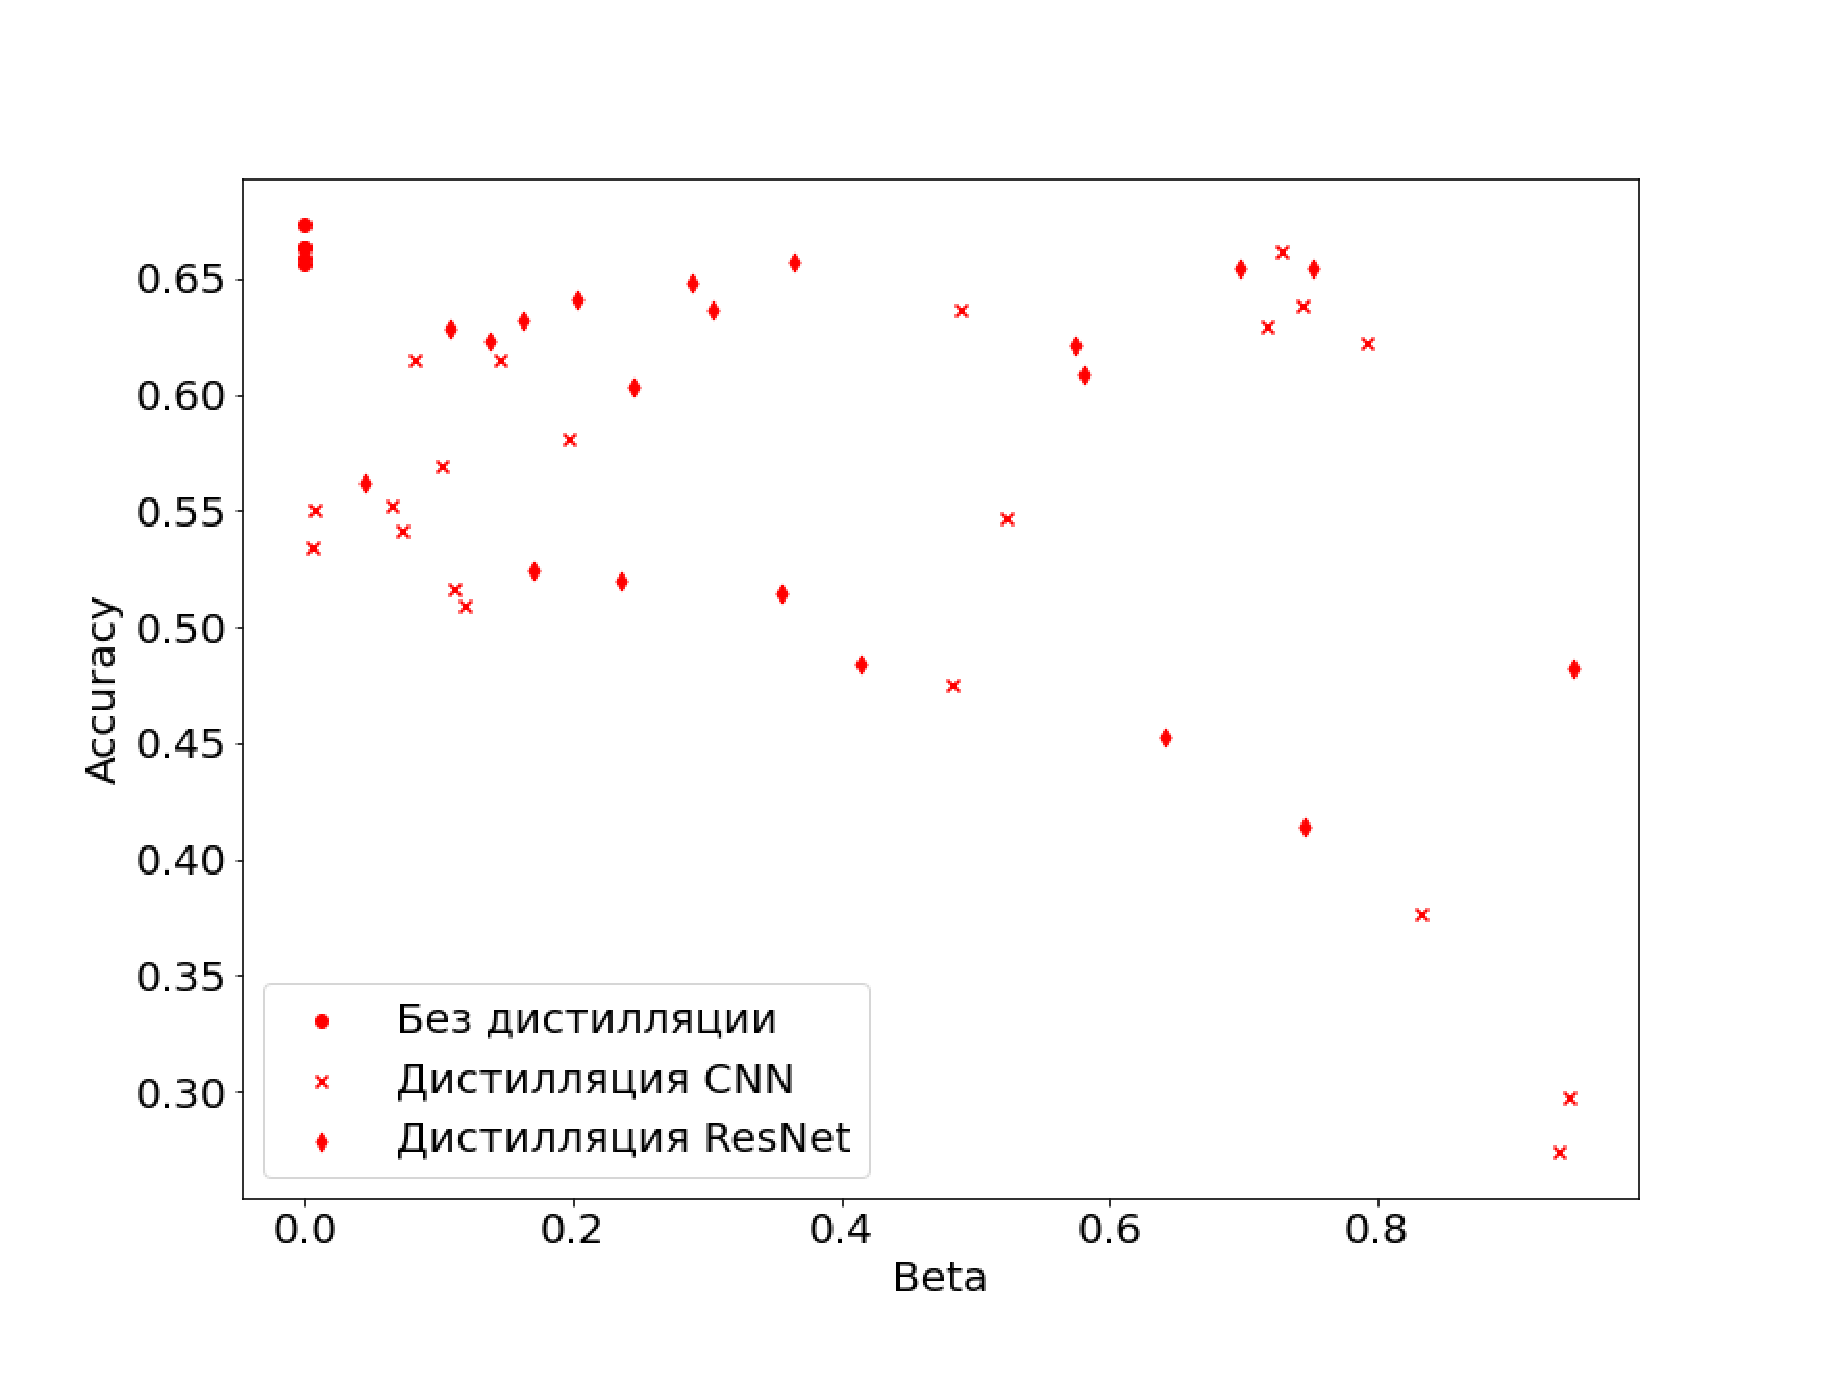
\includegraphics[width=0.5\textwidth]{scatter_beta_acc.eps}
    \caption{График зависимости точности от $\beta$}
    \label{fig:beta_acc}
\end{figure}

\begin{figure}[!ht]
    \centering
    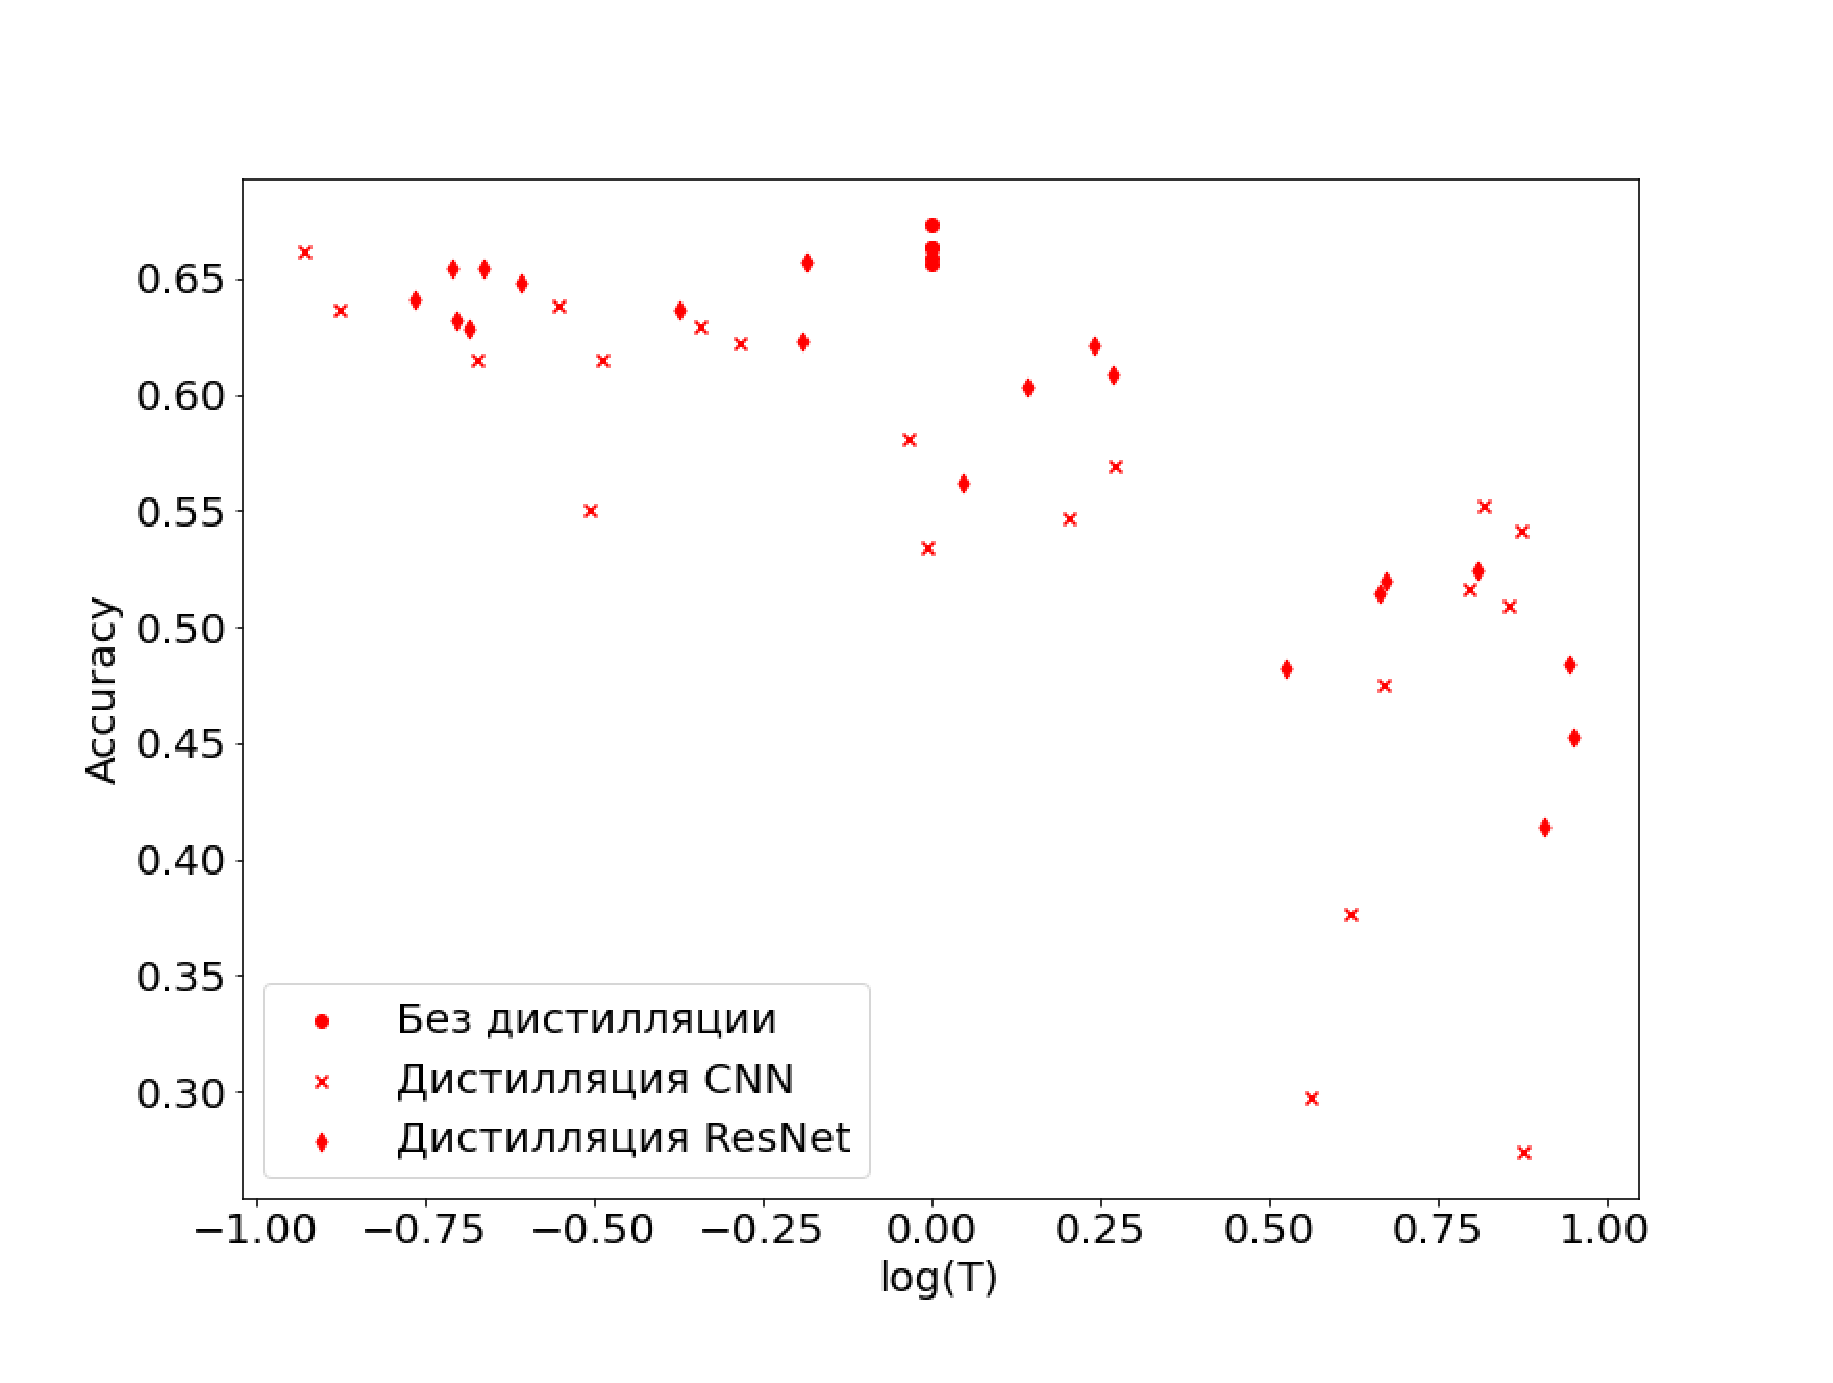
\includegraphics[width=0.5\textwidth]{scatter_temp_acc.eps}
    \caption{График зависимости точности от температуры}
    \label{fig:temp_acc}
\end{figure}

\begin{figure}[!ht]
    \centering
    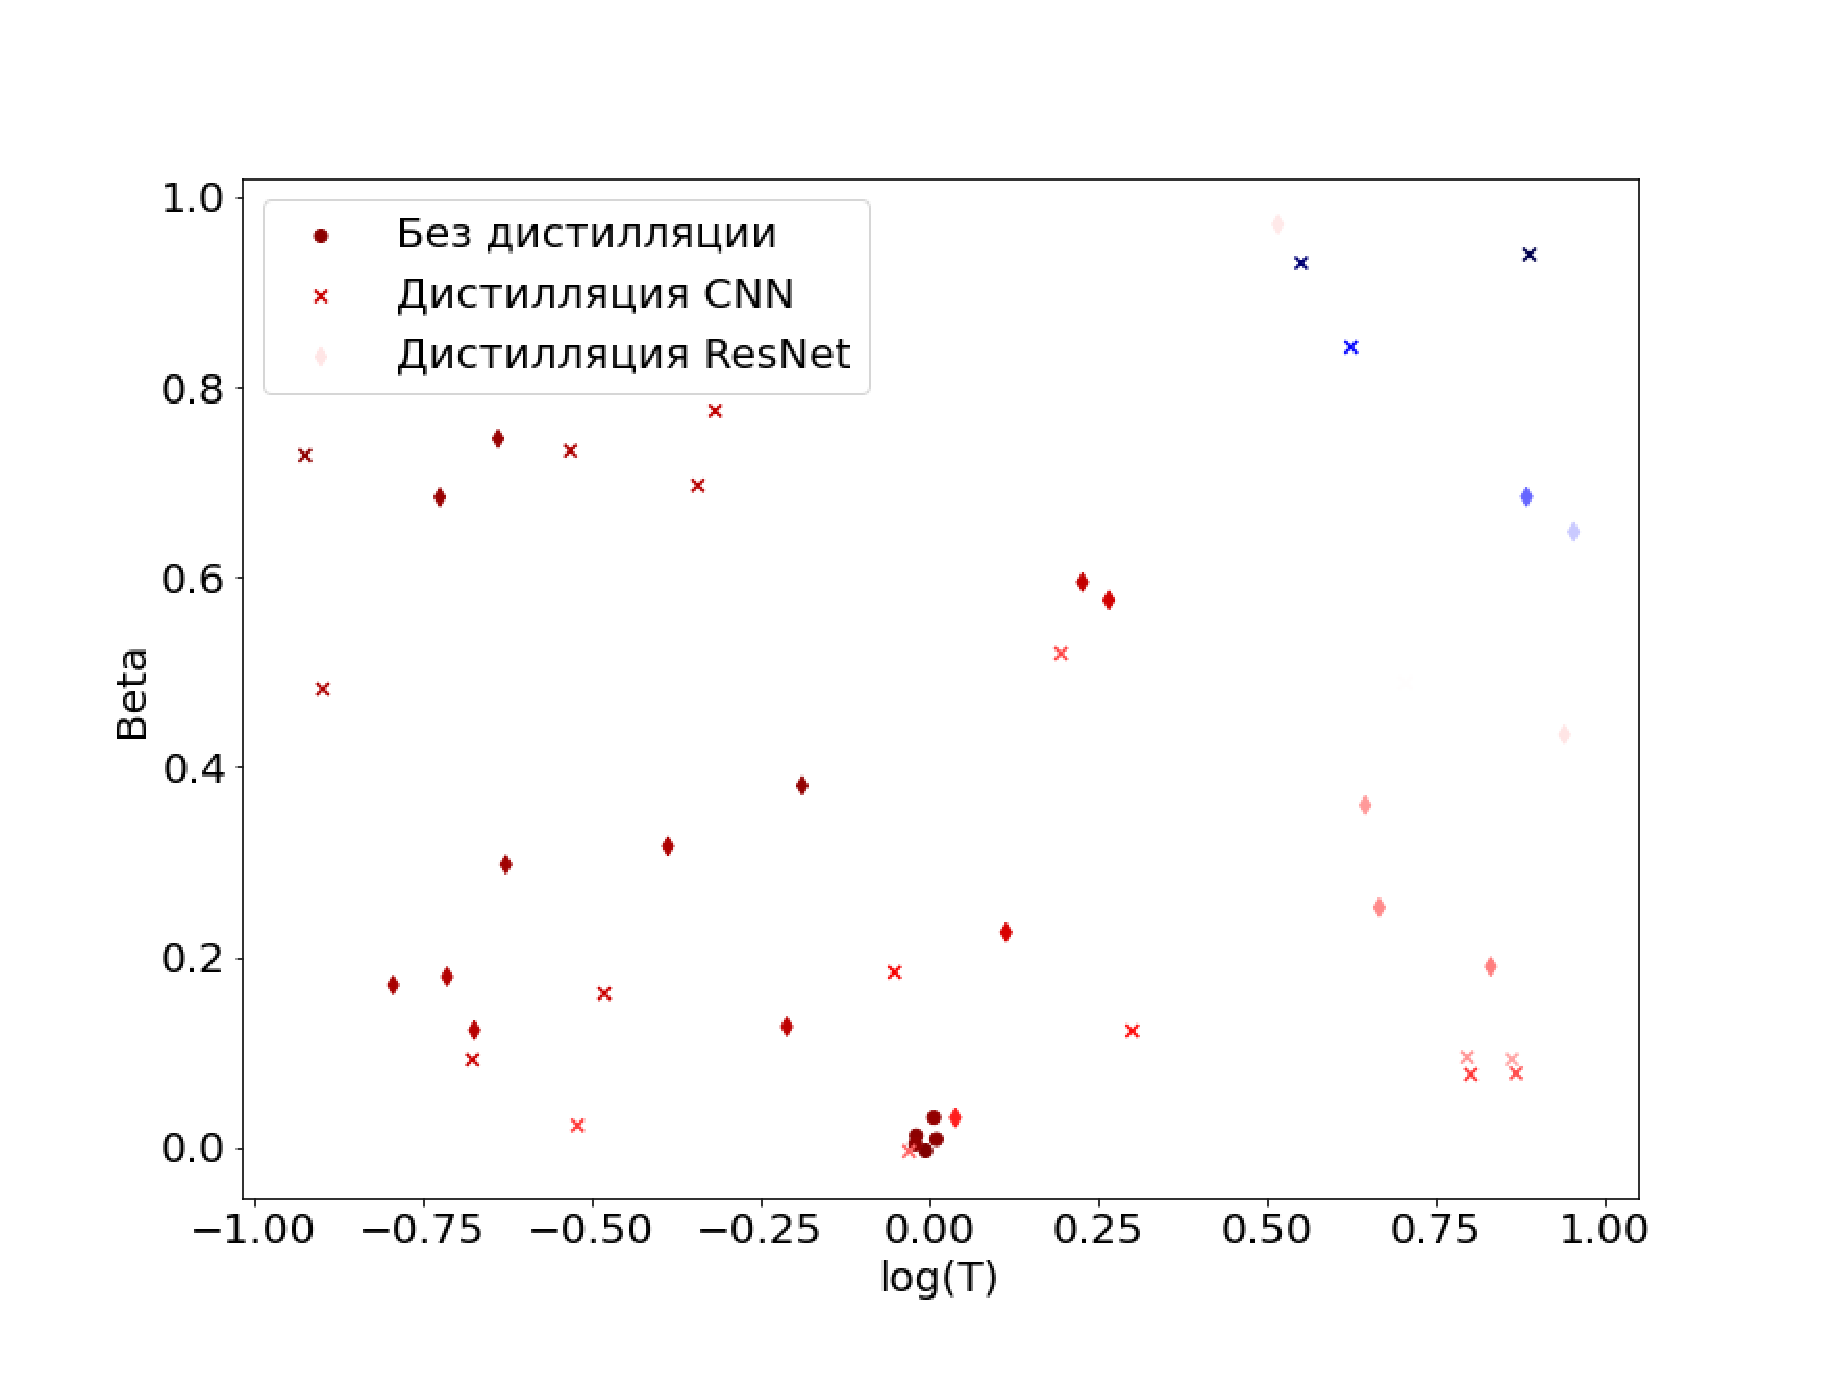
\includegraphics[width=0.5\textwidth]{scatter_temp_beta.eps}
    \caption{График зависимости $\beta$ от температуры с выделенной цветом $\text{accuracy}$}
    \label{fig:temp_beta}
\end{figure}

На~рис. \ref{fig:beta_acc} изображена зависимость точности от величины коэффициента $\beta$. Различные точки отвечают за точность модели без дистилляции, с дистилляцией ResNet и CNN. Можно заметить, что с уменьшением значения коэффициента $\beta$ значение точности увеличивается.

На~рис. \ref{fig:temp_acc} изображена зависимость точности от $T$. Для изображения значений температуры используется логарифмическая шкала. По графику видно, что значение температуры уменьшается при увеличении логарифма температуры, но при значениях логарифма от 0.5 до 1 наблюдается резкое уменьшение точности.

На~рис. \ref{fig:temp_beta} изображена зависимость $\beta$ от величины $T$ с выделенной цветом $\text{accuracy}$. Заметим, что точки с большим значением точности в основном расположены в правом нижнем углу графика, а именно, при значениях $\beta$ от 0 до 0.5 и значениях $\log(T)$ от -1 до 0. Наоборот, точки с низким значением точности, расположены в правом верхнем углу графика.

\begin{table}[h]
    \centering
    \begin{tabular}{c|c}
         &  \\
         & 
    \end{tabular}
    \caption{Результаты эксперимента}
    \label{tab:experiment_results}
\end{table}

В таблице \ref{tab:experiment_results} приведены результаты эксперимента.

\begin{figure}[h]
    \centering
    \caption{График зависимости $\beta$ от количества итераций дистилляции}
    \label{fig:iter_beta}
\end{figure}

\begin{figure}[h]
    \centering
    \caption{График зависимости температуры от количества итераций дистилляции}
    \label{fig:iter_temp}
\end{figure}

На~рис. \ref{fig:iter_beta} изображена зависимость $\beta$ от количества итераций дистилляции.

На~рис. \ref{fig:iter_temp} изображена зависимость $T$ от количества итераций дистилляции.

\paragraph{Название параграфа}
Разделы и~параграфы, за исключением списков литературы, нумеруются.

\section{Заключение}
Желательно, чтобы этот раздел был, причём он не~должен дословно повторять аннотацию.
Обычно здесь отмечают, каких результатов удалось добиться, какие проблемы остались открытыми.

%%%% если имеется doi цитируемого источника, необходимо его указать, см. пример в \bibitem{article}
%%%% DOI публикации, зарегистрированной в системе Crossref, можно получить по адресу http://www.crossref.org/guestquery/

\bibliographystyle{bibstyle.bst}
\bibliography{bibliography.bib}


%%%% если имеется doi цитируемого источника, необходимо его указать, см. пример в \bibitem{article}
%%%% DOI публикации, зарегистрированной в системе Crossref, можно получить по адресу http://www.crossref.org/guestquery/.

\end{document}
